\section{NeuroTechX loves DLEEG}
\NTXDivider{NeuroTechX\,$\heartsuit$\,DLEEG}

\begin{frame}{MOABB: making BCI comparisons reproducible}
  \begin{columns}[c,onlytextwidth]
    \column{.43\textwidth}
      \small
      \NTXPoint{Mother of All BCI Benchmarks}{Open comparisons on public EEG datasets.}
      \NTXPoint{The 2024 benchmark study}{30 pipelines, 36 datasets:\newline motor imagery, P300, and SSVEP.}
      \NTXPoint{A shared research foundation}{Implementations and evaluations others can inspect and reproduce.}
    \column{.53\textwidth}
      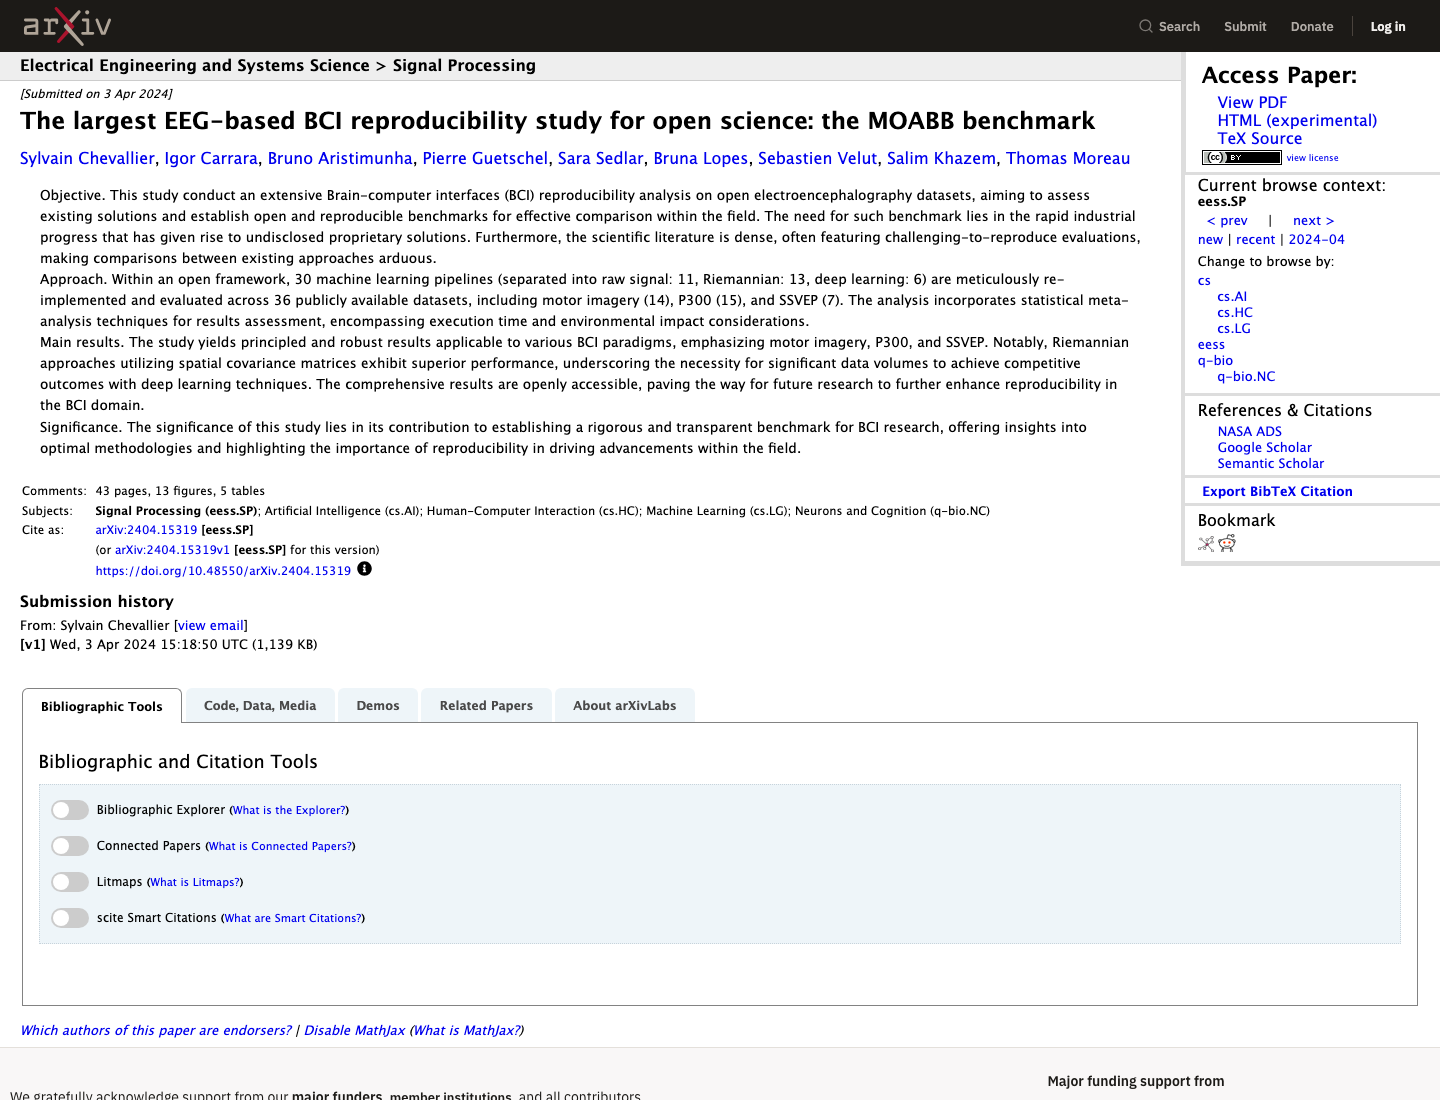
\includegraphics[width=\linewidth,height=45mm,keepaspectratio]{assets/history/moabb-arxiv-abstract.png}
      \par\smallskip{\scriptsize The MOABB benchmark --- arXiv abstract page\par}
  \end{columns}
  \NTXSource{https://arxiv.org/abs/2404.15319}{Chevallier et al., 2024, arXiv:2404.15319}
  \note{[36:45--38:15] MOABB is an example of community work producing a research artifact beyond a single event. The numerical scope is specific to the cited 2024 study, not today's dataset total. Credit the contributors. Do not generalize the study into a claim that a particular algorithm always wins or that benchmark performance establishes clinical utility.}
\end{frame}

\begin{frame}{Shared tools, shared teaching: a path into DLEEG}
  \begin{columns}[c,onlytextwidth]
    \column{.58\textwidth}
      \small
      \NTXPoint{An interoperable Python ecosystem}{MNE: EEG processing. scikit-learn: pipelines and evaluation. pyRiemann: covariance-based learning.}
      \NTXPoint{Pedro Rodrigues and Sylvain Chevallier}{Hands-on teaching with reusable notebooks: \href{https://github.com/plcrodrigues/Workshop-MOABB-BCI-Graz-2019}{Graz 2019} and the \href{https://github.com/mccorsi/BCI-2023-Open-Source-Tool-workshop}{2023 open-source BCI workshop}.}
      \NTXPoint{The next generation carries it forward}{Istanbul, MLSP 2025: Bruno Aristimunha co-organized with Sylvain, Florian Yger, and Marie-Constance Corsi.}
    \column{.38\textwidth}
      \centering
      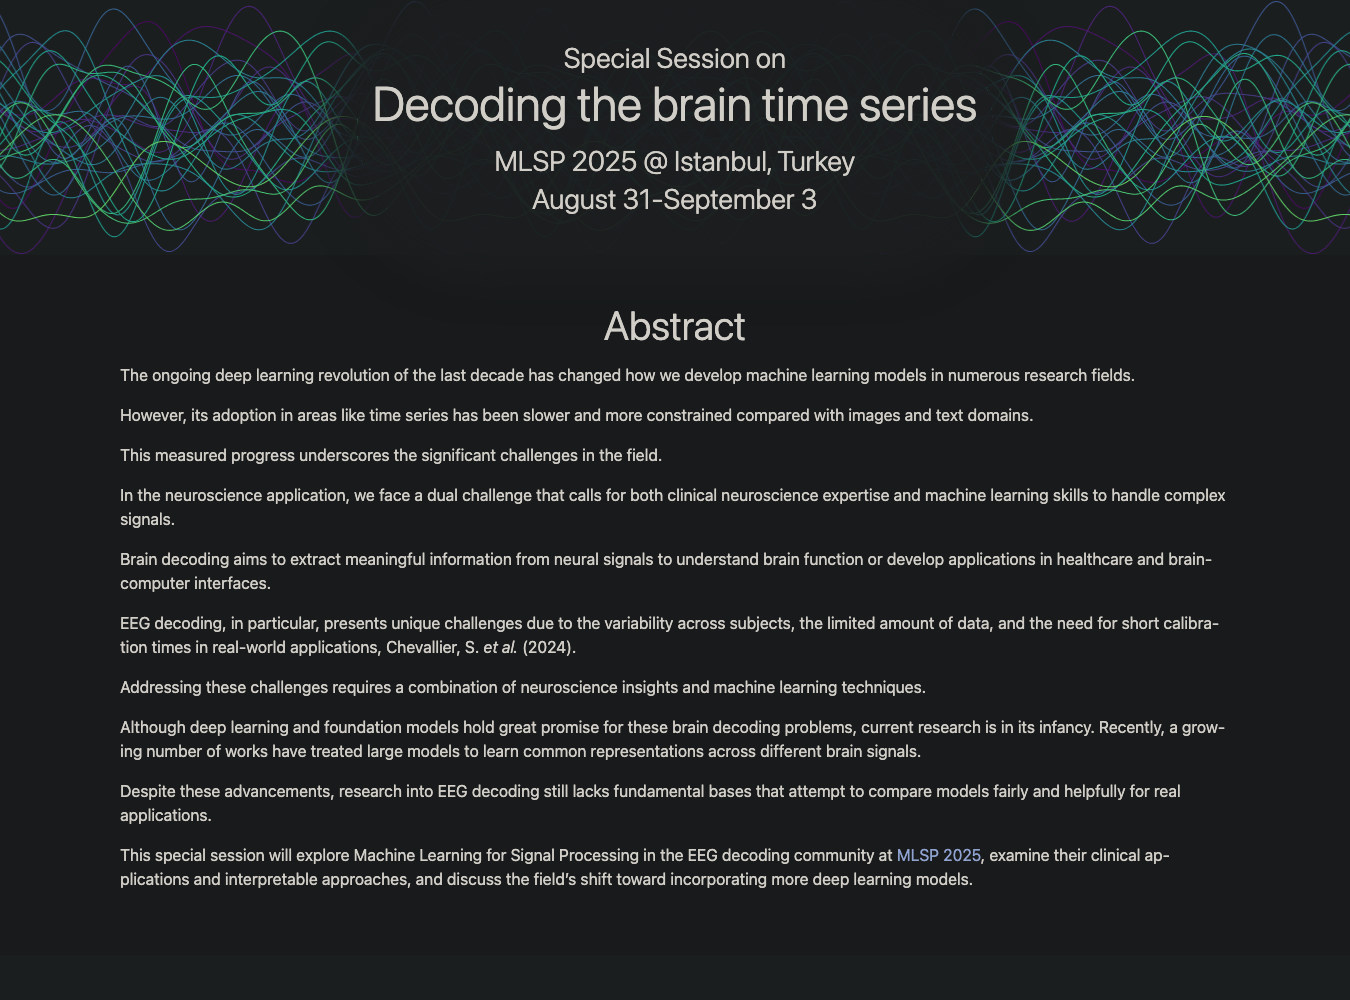
\includegraphics[width=\linewidth,height=42mm,keepaspectratio]{assets/history/dleeg-istanbul-workshop.png}\par\smallskip
      {\tiny Decoding the brain time series\newline Istanbul, August 31--September 3, 2025\newline Official special-session page\par}
  \end{columns}
  {\tiny\color{NTXMuted}Sources: linked workshop repositories; \href{https://mlsp2025-decoding-brain.github.io/}{MLSP 2025}; \href{https://bruaristimunha.github.io/}{Bruno Aristimunha}. DLEEG = deep learning for EEG.\par}
  \note{[38:15--39:45] Start with the ecosystem that makes rigorous EEG machine learning teachable. MNE handles EEG data and preprocessing; scikit-learn supplies reusable estimators, pipelines, and evaluation; pyRiemann brings covariance geometry into this ecosystem. These are broader than deep learning and provide useful baselines. Pedro is Pedro L. C. Rodrigues. His Graz 2019 repo explicitly teaches these tools with MOABB. The 2023 workshop lists Sylvain on MOABB and Pedro on pyRiemann; do not attribute every workshop exclusively to them. Also see the lkorczowski/BCI-2021-Riemannian-Geometry-workshop repository. Istanbul was a special session within IEEE MLSP 2025, not a standalone NTX training workshop. Its organizers include Bruno, Florian, Marie-Constance, and Sylvain; Hubert Banville was the announced keynote speaker. Bruno's own biography identifies Sylvain, Marie-Constance, and Raphael de Camargo as his PhD advisors. He illustrates the next generation; do not label all co-organizers as Sylvain's students or assert that NTX owns these libraries.}
\end{frame}

\begin{frame}{Yannick Roy and colleagues: mapping deep learning for EEG}
  \begin{columns}[c,onlytextwidth]
    \column{.47\textwidth}
      \small
      \NTXPoint{A systematic review, 2019}{\emph{Deep learning-based electroencephalography analysis: a systematic review.}}
      \NTXPoint{Across application areas}{Epilepsy, sleep, BCI, and cognitive and affective monitoring.}
      \NTXPoint{A community research agenda}{Share data and code; strengthen reproducibility and comparisons between methods.}
    \column{.49\textwidth}
      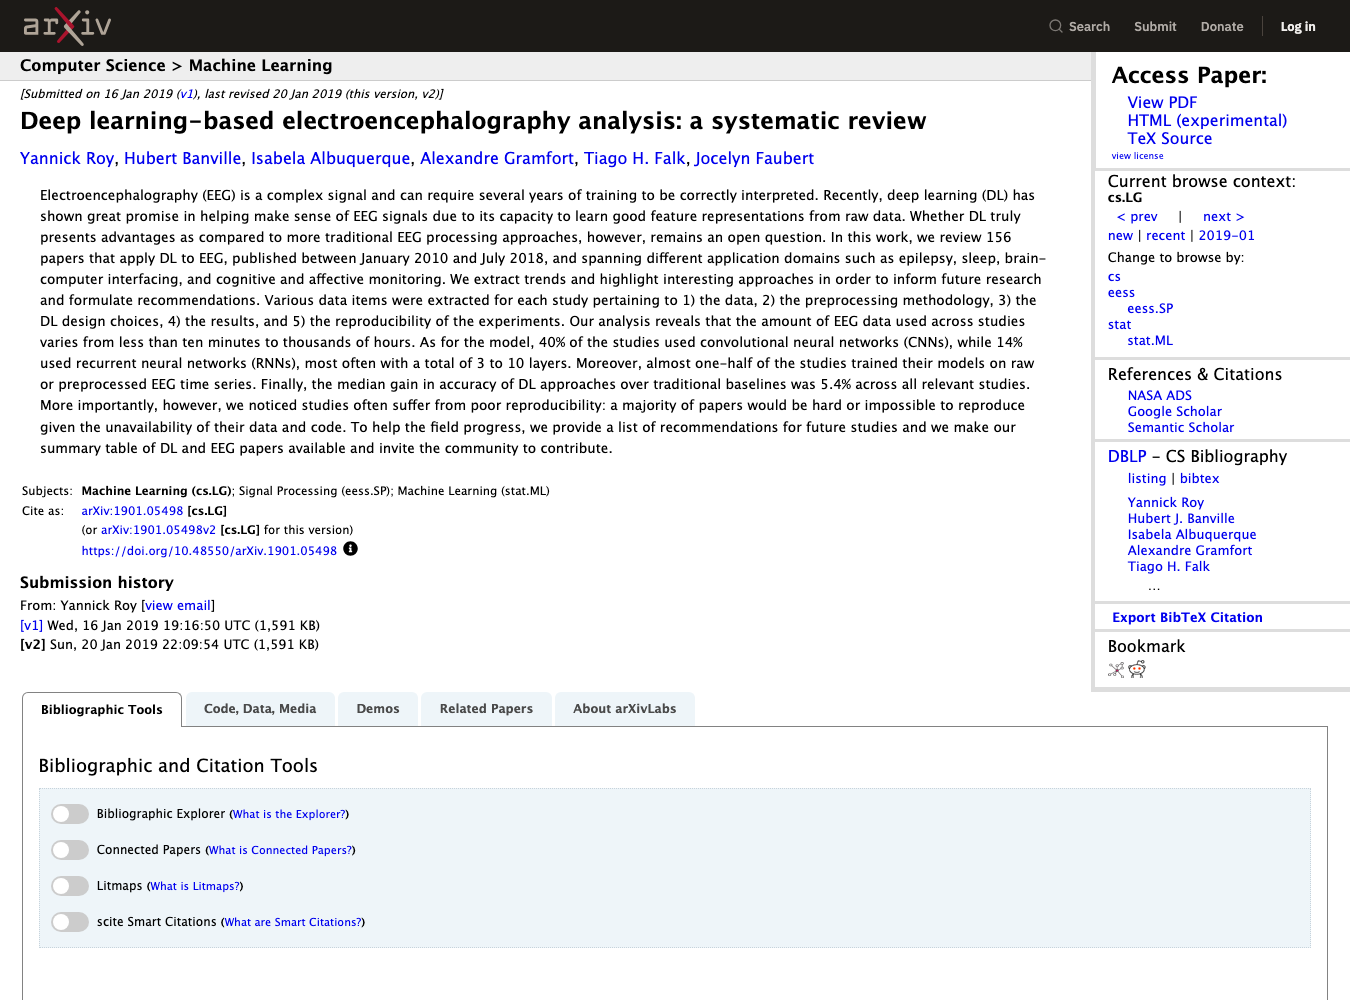
\includegraphics[width=\linewidth,height=45mm,keepaspectratio]{assets/history/dleeg-roy-article-page.png}\par\smallskip
      {\tiny Article's arXiv abstract page\newline Roy, Banville, Albuquerque, Gramfort, Falk, Faubert\par}
  \end{columns}
  {\tiny\color{NTXMuted}Sources: \href{https://arxiv.org/abs/1901.05498}{arXiv:1901.05498}; \href{https://doi.org/10.1088/1741-2552/ab260c}{Journal of Neural Engineering 16, 051001 (2019)}\par}
  \note{[39:45--41:15] Credit all authors: Yannick Roy, Hubert Banville, Isabela Albuquerque, Alexandre Gramfort, Tiago H. Falk, and Jocelyn Faubert. The review covers work published from January 2010 to July 2018 and emphasizes reproducibility and data/code availability. The displayed image is a genuine arXiv article-page screenshot, not the journal publisher's page. Its preprint abstract reports 156 papers; the published abstract indexed in PubMed reports 154, so the slide deliberately does not mix counts across versions. This is a review and research agenda, not a new model or evidence that deep learning always beats classical pipelines. Connect Yannick's work with the workshops and open tools without inventing a formal causal relationship between the review and later challenges.}
\end{frame}

\begin{frame}{Neureka 2020: community, clinical EEG, shared evaluation}
  \begin{columns}[c,onlytextwidth]
    \column{.58\textwidth}
      \small
      \NTXPoint{NeuroTechX + Novela Neurotech}{A global epilepsy challenge built around automatic seizure detection.}
      \NTXPoint{The TUH corpus team}{Joseph Picone and colleagues at Temple's Neural Engineering Data Consortium: TUH seizure data and open scoring tools.}
      \NTXPoint{A challenge becomes research}{19 teams; 16 scorable submissions. The team studied how scoring choices affect evaluation.}
    \column{.38\textwidth}
      \centering
      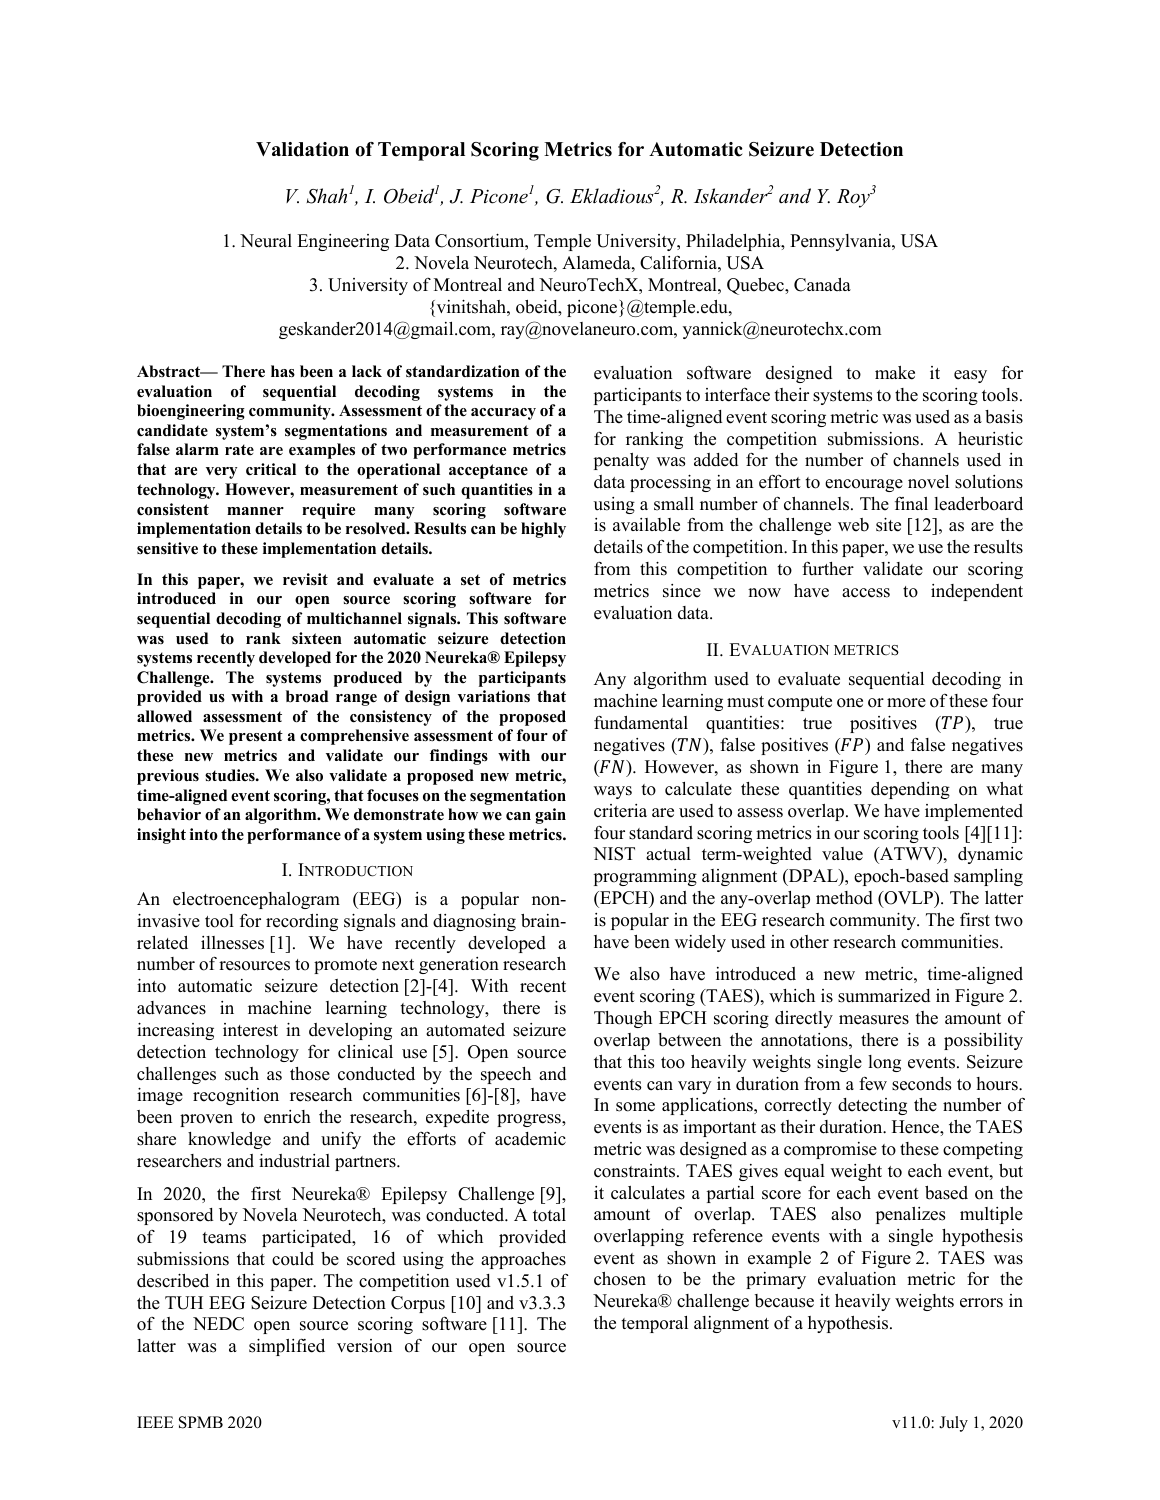
\includegraphics[width=\linewidth,height=46mm,keepaspectratio]{assets/history/neureka-scoring-first-page.png}\par\smallskip
      {\tiny Shah, Obeid, Picone, Ekladious, Iskander, Roy\newline IEEE SPMB 2020 scoring study\par}
  \end{columns}
  {\tiny\color{NTXMuted}Sources: \href{https://sccn.ucsd.edu/pipermail/eeglablist/2020/014884.html}{Yannick's challenge announcement}; \href{https://isip.piconepress.com/conferences/ieee_spmb/2020/papers/l02_05.pdf}{Validation of Temporal Scoring Metrics for Automatic Seizure Detection}\par}
  \note{[41:15--42:45] NeuroTechX and Novela Neurotech launched the challenge in 2020. The subsequent scoring paper lists Vinit Shah, Iyad Obeid, Joseph Picone, Georges Ekladious, Ray Iskander, and Yannick Roy; its affiliations link Temple's NEDC, Novela, and NeuroTechX. It reports 19 participating teams and 16 scorable systems using TUH EEG Seizure Detection Corpus v1.5.1 and NEDC scoring software v3.3.3. Say seizure detection, not prospective seizure prediction or diagnosis. The example belongs in the broader EEG machine-learning story: the challenge was not restricted to deep neural networks. Patient-separated train/development/evaluation sets and sensitivity to scoring choices illustrate why shared data need shared evaluation. No claim of approved clinical deployment, open patient-data redistribution, or exclusive NTX authorship of TUH.}
\end{frame}

% Existing benchmark, toolkit, methods-community and foundation-challenge frames follow.
\begin{frame}{Braindecode: deep learning joins the shared toolkit}
  \begin{columns}[c,onlytextwidth]
    \column{.45\textwidth}
      \small
      \NTXPoint{2017: deep learning for EEG}{Schirrmeister et al.: ConvNets and open-source Braindecode.}
      \NTXPoint{A connected research toolkit}{PyTorch, MNE, MOABB datasets, and pretrained models.}
      \NTXPoint{From classical baselines to learned features}{Train neural decoders within a reproducible EEG workflow.}
    \column{.51\textwidth}
      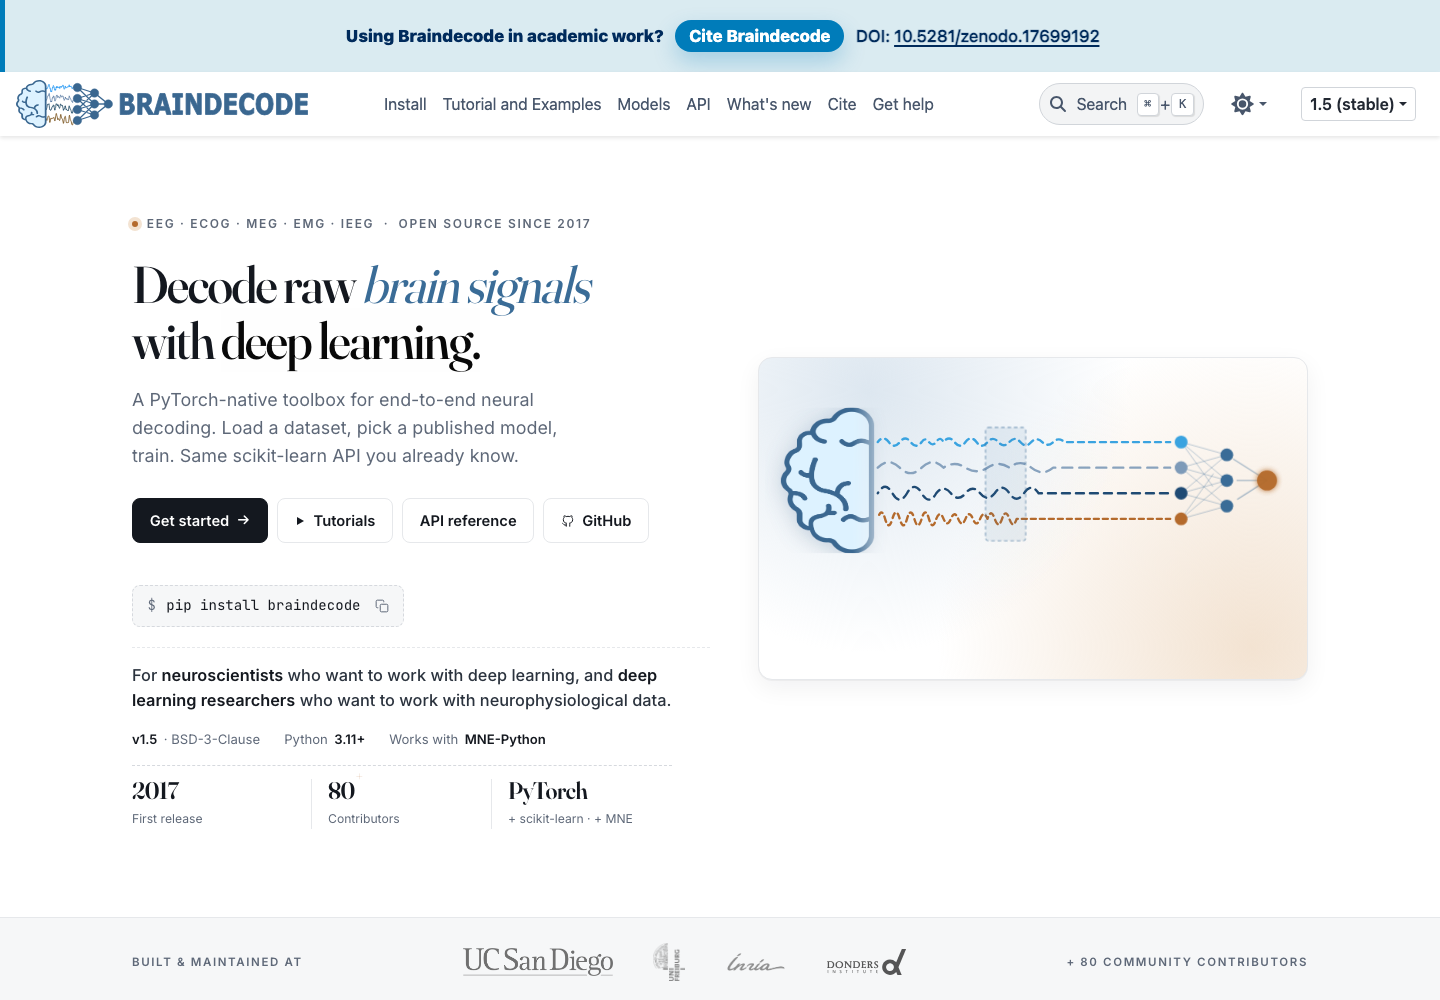
\includegraphics[width=\linewidth,height=45mm,keepaspectratio]{assets/history/braindecode-homepage.png}
      \par\smallskip{\scriptsize Braindecode's official project homepage\par}
  \end{columns}
  {\tiny\color{NTXMuted}Sources: \href{https://doi.org/10.1002/hbm.23730}{Schirrmeister et al., 2017}; \href{https://braindecode.org/stable/}{Braindecode}; \href{https://github.com/braindecode/OpenEEGBench}{Guetschel et al., OpenEEG-Bench, 2026}\par}
  \note{[42:45--44:15] Braindecode's foundational paper is Schirrmeister et al., Deep learning with convolutional neural networks for EEG decoding and visualization, Human Brain Mapping 2017, doi:10.1002/hbm.23730. Current documentation describes PyTorch/MNE integration and access to MOABB and pretrained models. OpenEEG-Bench is a distinct benchmark under the Braindecode organization, not a renamed MOABB or the NeurIPS competition itself. Guetschel, Aristimunha, Truong, Kokate, Tangermann, and Delorme's Toward OpenEEG-Bench paper builds explicitly on organizing the NeurIPS 2025 EEG Foundation Model Challenge. Its initial study covers five models and ten datasets. The current repository lists twelve datasets and probing, parameter-efficient adaptation, and full fine-tuning options. Do not mix those scopes or give an unverified current leaderboard ranking. Community contribution here means testing models under comparable preprocessing, splits, and adaptation procedures; not claiming NTX owns these projects.}
\end{frame}


\begin{frame}{OpenEEG-Bench: how should we adapt foundation models?}
  \begin{columns}[c,onlytextwidth]
    \column{.49\textwidth}
      \small
      \NTXPoint{A community-driven benchmark}{Compare EEG foundation models with shared data and evaluation pipelines.}
      \NTXPoint{Adaptation is part of the question}{Frozen-encoder probes, parameter-efficient adaptation, and full fine-tuning are different tests.}
      \NTXPoint{A contribution chapters can make}{Reproduce baselines, test new datasets, and report both accuracy and training cost.}
    \column{.47\textwidth}
      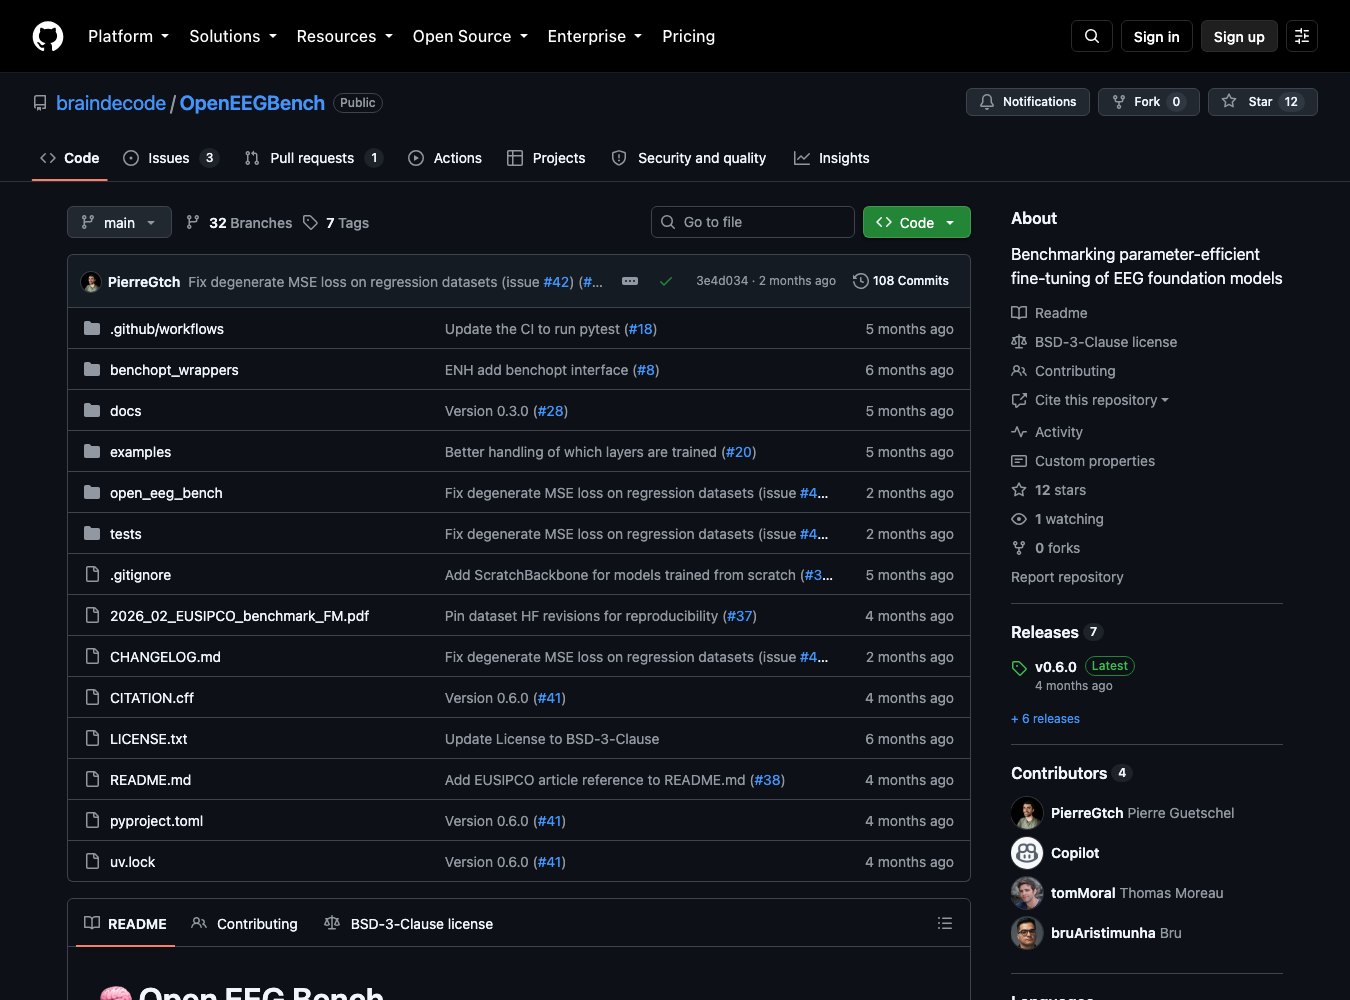
\includegraphics[width=\linewidth,height=43mm,keepaspectratio]{assets/history/openeegbench-repository.png}\par\smallskip
      {\tiny OpenEEG-Bench / Braindecode GitHub organization\par}
  \end{columns}
  \NTXSource{https://github.com/braindecode/OpenEEGBench}{Guetschel and colleagues, OpenEEG-Bench, 2026}
  \note{[44:15--45:45] This dedicated slide separates the benchmark from the Braindecode software history. The initial Toward OpenEEG-Bench paper evaluated five models on ten datasets; the evolving repository has a different scope. Avoid presenting either number as a permanent total. The current code supports frozen encoders, ridge probes, low-rank and other parameter-efficient approaches, full fine-tuning and two-stage adaptation. These answer different questions and must not be pooled into an undifferentiated leaderboard. Community contribution is our proposed use of the project, not a claim of NTX ownership or an established chapter program.}
\end{frame}

\begin{frame}{NeuroAtlas: a reality check for EEG foundation models}
  \begin{columns}[c,onlytextwidth]
    \column{.57\textwidth}
      \small
      \NTXPoint{KU Leuven + MIT, 2026}{42 datasets; approximately 260,000 hours across epilepsy, sleep, brain age, and BCI.}
      \NTXPoint{What transfers from a frozen model?}{EEG foundation models, generic time-series foundation models, and supervised-pretrained baselines.}
      \NTXPoint{No consistent EEG-specific advantage}{Rankings vary across datasets and metrics; an out-of-the-box universal EEG model remains a goal.}
    \column{.39\textwidth}
      \centering
      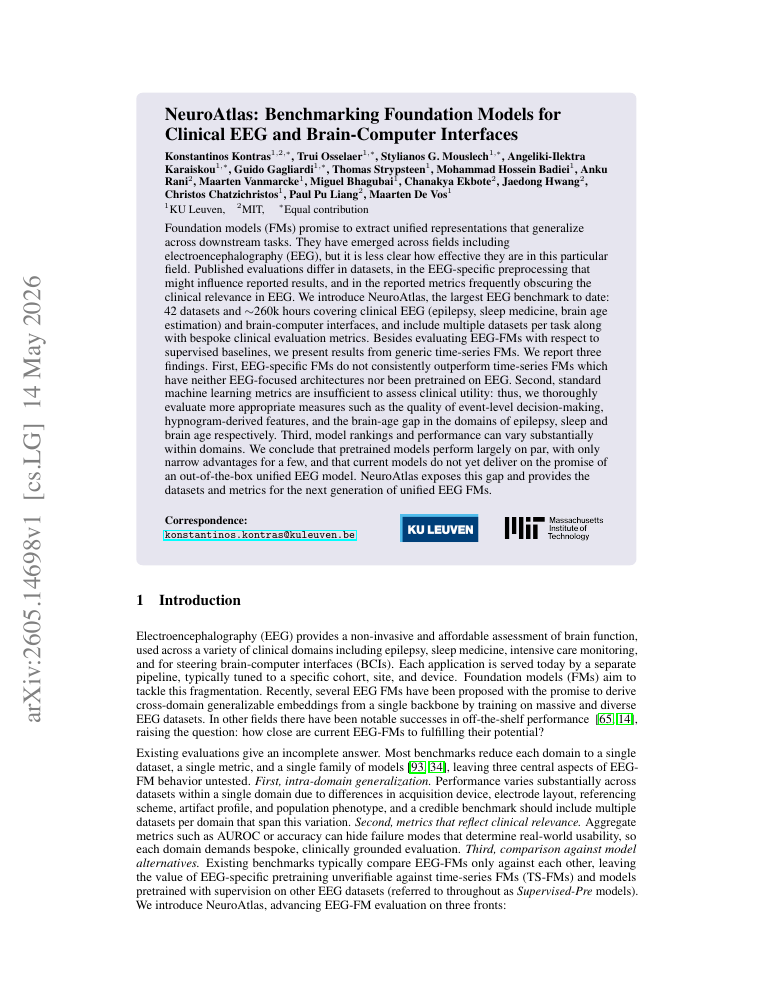
\includegraphics[width=\linewidth,height=46mm,keepaspectratio]{assets/history/neuroatlas-first-page.png}\par\smallskip
      {\tiny Kontras and colleagues, May 2026 preprint\par}
  \end{columns}
  \NTXSource{https://arxiv.org/abs/2605.14698}{NeuroAtlas: Benchmarking Foundation Models for Clinical EEG and Brain-Computer Interfaces}
  \note{[45:45--47:15] NeuroAtlas is the MIT/KU Leuven project Morgan confirmed, not NeuroSTORM. Its frozen-encoder protocol fits downstream probes rather than fully fine-tuning each backbone. The comparison includes supervised-pretrained neural models, not just classical non-neural pipelines. EEG-specific pretraining did not consistently beat generic time-series pretraining. Clinical-task metrics can change conclusions drawn from standard accuracy scores. This is a May 2026 preprint and a scoped benchmark, not proof that all foundation models fail or that any model is clinically ready.}
\end{frame}

\begin{frame}{Do NeuroFMs beat classical methods?}
  \begin{columns}[c,onlytextwidth]
    \column{.54\textwidth}
      \small
      \NTXPoint{Not consistently}{With scarce BCI data, gains over compact networks or classical decoders are often not significant.}
      \NTXPoint{Fine-tuning can change the result}{Data-rich settings can favor fine-tuned models. Frozen probing is a different test.}
      \NTXPoint{Keep the classical baseline}{Compare on the same task and splits, with uncertainty, calibration needs, and compute cost.}
    \column{.42\textwidth}
      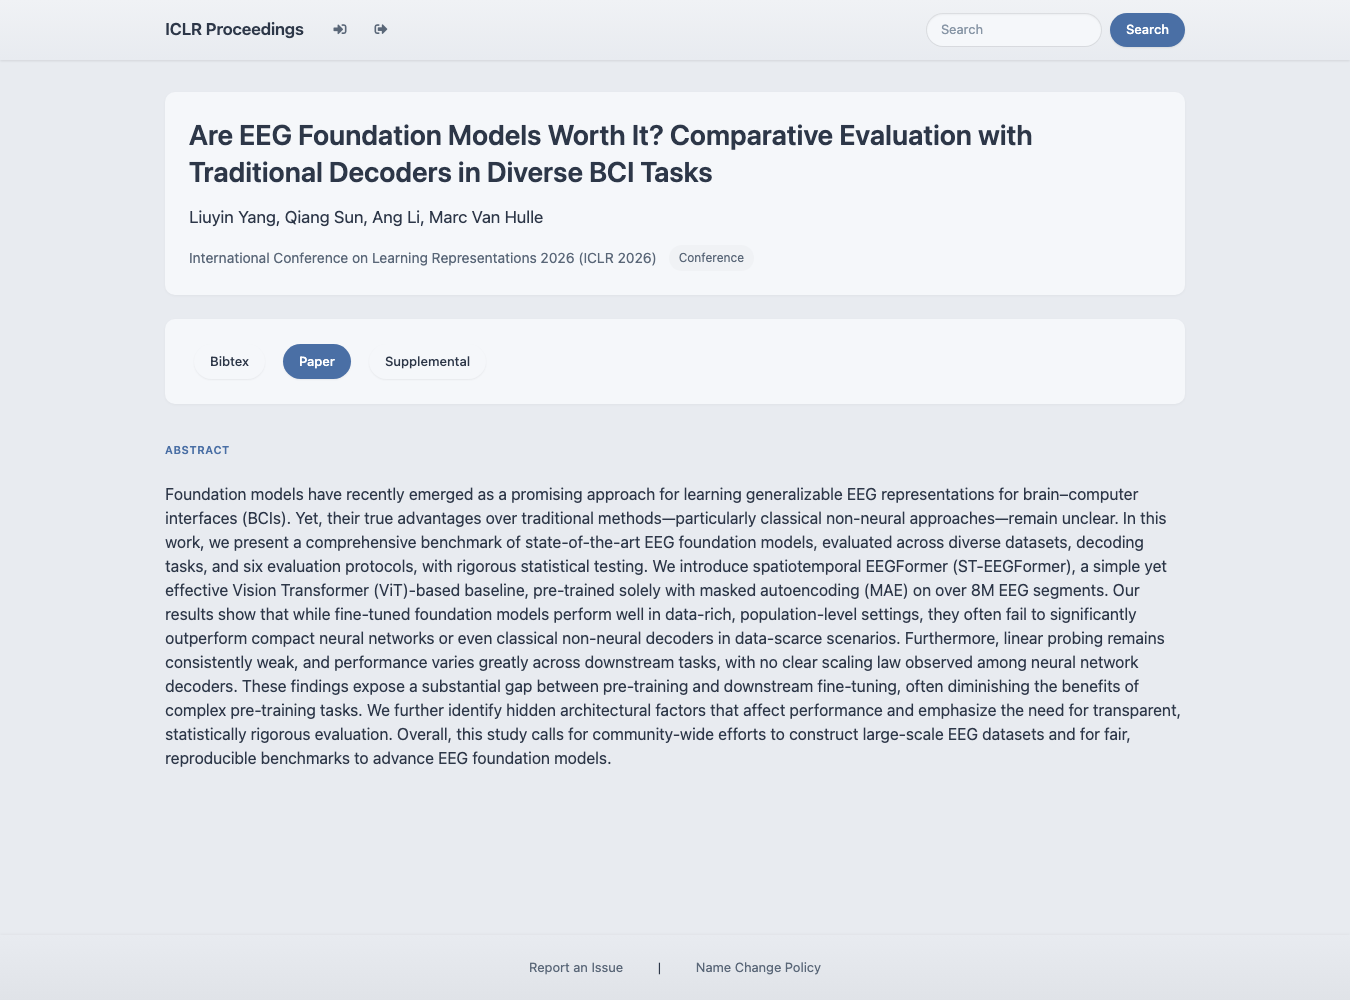
\includegraphics[width=\linewidth,height=43mm,keepaspectratio]{assets/history/eeg-fms-worth-it-page.png}\par\smallskip
      {\tiny Yang, Sun, Li, Van Hulle / ICLR 2026\newline Official proceedings abstract page\par}
  \end{columns}
  {\tiny\color{NTXMuted}Sources: \href{https://proceedings.iclr.cc/paper_files/paper/2026/hash/f0f39b7686634fc81ca0112566b2c05f-Abstract-Conference.html}{Are EEG Foundation Models Worth It?}; \href{https://github.com/LiuyinYang1101/STEEGFormer}{code and benchmark}\par}
  \note{[47:15--48:45] This separate ICLR 2026 study directly compares foundation models with traditional BCI decoders across six evaluation protocols. It supports a conditional answer, not a blanket claim that classical methods win. The authors report stronger foundation-model results with full fine-tuning and sufficient data, but frequently no significant advantage in data-scarce settings. Compact neural networks are distinct from classical non-neural methods. These experiments and NeuroAtlas have different protocols and cannot be merged into a single ranking. Our takeaway is to move into deep learning without discarding rigorous classical baselines. Cost and calibration reporting are our evaluation recommendations, not numerical results asserted from this paper.}
\end{frame}

\begin{frame}{CuttingGardens: global methods, local communities}
  \begin{columns}[c,onlytextwidth]
    \column{.55\textwidth}
      \small
      \NTXPoint{2023: the first distributed edition}{Shared M/EEG lectures; local tutorials, discussions, and networking.}
      \NTXPoint{2025: studying the conference model}{Published evaluation of ecological and social sustainability.}
      \NTXPoint{Next: 21--25 September 2026}{A broadcast global program with local activities around the world.}
    \column{.41\textwidth}
      \centering
      
\includegraphics[width=\linewidth,height=46mm,keepaspectratio]{assets/history/cuttinggardens-2026.png}
      \par\smallskip{\scriptsize Official 2026 event artwork\par}
  \end{columns}
  {\tiny\color{NTXMuted}Sources: \href{https://cuttinggardens2023.org/}{CuttingGardens 2023}; \href{https://doi.org/10.1371/journal.pstr.0000177}{Corneyllie et al., 2025}; \href{https://cuttingeeg.org/cuttinggardens2026/}{CuttingGardens 2026}\par}
  \note{[48:45--50:15] CuttingGardens is part of the CuttingEEG conference series, not an NTX event or a Braindecode project. The 2023 meeting introduced distributed local hubs connected by a common program. Corneyllie, Walters, Chaumon and colleagues published Doing conferences differently: A decentralised multi-hub approach for ecological and social sustainability in PLOS Sustainability and Transformation on June 23, 2025, doi:10.1371/journal.pstr.0000177. The paper reports 21 hubs, 730 in-person and 300 online attendees for 2023; these are retrospective figures, not 2026 forecasts. The upcoming global meeting is September 21--25, 2026. Local dates and activities vary. The 2026 site contains inconsistent hub/continent totals, so none are asserted. The connection to NTX is a model for distributed methods education and participation, not a formal partnership claim.}
\end{frame}

\begin{frame}{From global hackathons to foundation-model challenges}
  \begin{columns}[c,onlytextwidth]
    \column{.52\textwidth}
      \small
  \NTXPoint{Global hackathons}{A community coming together around shared technical challenges.}
  \NTXPoint{2025: EEG Foundation Challenge}{Cross-task and cross-subject decoding.\newline NeurIPS competition; results highlighted at SfN.}
  \NTXPoint{2026: EEG/EMG Foundation Challenge}{Four tracks testing generalization across brain and body signals.\newline Winners present at the NeurIPS Brain and Body workshop.}
    \column{.44\textwidth}
      \centering
      {\small\textbf{2025 EEG $\longrightarrow$ 2026 EEG / EMG}\par}\medskip
      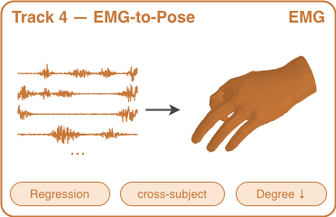
\includegraphics[width=\linewidth,height=33mm,keepaspectratio]{assets/history/challenge2026-emg-to-pose.png}\par\smallskip
      {\scriptsize A new brain-and-body task: EMG-to-pose\newline Official 2026 challenge illustration\par}
  \end{columns}
  {\tiny\color{NTXMuted}Sources: \href{https://eeg2025.github.io/}{EEG 2025}; \href{https://sccn.ucsd.edu/pipermail/eeglablist/2025/018754.html}{SCCN at SfN}; \href{https://neural-interfaces26.github.io/}{EEG/EMG 2026}; \href{https://brainbodyfm-workshop.github.io/}{Foundation Models for the Brain and Body}\par}
  \note{[50:15--51:45] Morgan describes this as a progression from the global hackathon community into larger research challenges. The 2025 competition was part of NeurIPS; SCCN's November 2025 SfN booth announcement invited discussion of its results. The 2026 challenge covers image retrieval from EEG, BCI decoding, sleep onset, and hand pose from EMG. Its website says winners will present at Foundation Models for the Brain and Body at NeurIPS. This is upcoming, not a completed event. The challenge site credits promotion via NeuroTechX, EEGLAB, and MNE-Python. Distinguish Morgan's community-history account from formal event ownership; do not imply NTX exclusively organized all these programs.}
\end{frame}

\begin{frame}{Toward a MindEye-style EEG reconstruction project}
  \begin{columns}[c,onlytextwidth]
    \column{.48\textwidth}
      \small
      \NTXPoint{Alljoined: public data + model code}{Alljoined-1.6M: 1.6M+ EEG-image trials, 20 participants. ENIGMA: EEG-to-image reconstruction.}
      \NTXPoint{An ambitious chapter project}{Reproduce the results, then work toward a live EEG-to-image demonstration.}
      \NTXPoint{A direction, not yet equivalence}{MindEye's real-time demonstration uses fMRI. ENIGMA's reported EEG results average repeated trials.}
    \column{.48\textwidth}
      \includegraphics[page=6,trim=52 340 65 80,clip,width=\linewidth,height=43mm,keepaspectratio]{assets/history/enigma-2026.pdf}\par\smallskip
      {\tiny ENIGMA, Fig. 3: authors' selected best-scoring outputs\newline Seen images, not imagined scenes\par}
  \end{columns}
  {\tiny\color{NTXMuted}Sources: \href{https://huggingface.co/datasets/Alljoined/Alljoined-1.6M}{Dataset (CC BY-NC-SA 4.0)}; \href{https://github.com/Alljoined/ENIGMA}{ENIGMA code}; \href{https://arxiv.org/abs/2602.10361}{Kneeland et al., 2026}; \href{https://arxiv.org/abs/2607.22753}{Real-time MindEye2 adaptation, 2026}\par}
  \note{[51:45--53:15] This is Morgan's proposed direction for ambitious community projects, not an announcement of an NTX deployment or a demonstrated EEG port of MindEye. Alljoined publicly provides a large consumer-hardware EEG-image dataset and ENIGMA training, inference, and evaluation code. Public availability does not imply unrestricted commercial reuse: the dataset card specifies CC BY-NC-SA 4.0. We have not verified a pretrained checkpoint release. ENIGMA reconstructs viewed stimuli using a shared EEG encoder and generative image model. Appendix A.1 reports averaging 80 repetitions per inference sample; Figure 3 selects the highest-scoring sampled outputs. These are not typical single-trial live results or literal readouts of imagination. Iyer and colleagues' July 2026 real-time MindEye2 adaptation uses fMRI and RT-Cloud. The opportunity is to reproduce EEG baselines, test held-out images and people, and measure end-to-end latency and single-trial performance before calling a system real-time.}
\end{frame}
